

\documentclass[12pt]{article}

%\pagestyle{empty} 
\usepackage{amsmath}
\usepackage{algpseudocode}
\usepackage{algorithm}
\usepackage[english]{babel}
\usepackage{amsthm}
\usepackage{amssymb}
\usepackage{color}
\usepackage{graphicx}
\usepackage{epsfig}

\newcommand{\vs}{\vspace{2mm}}
\newcommand{\ls}{\vspace{5mm}} 

\newcommand{\ms}{\vspace{3mm}}
\newcommand{\bc}{\begin{center}}
\newcommand{\ec}{\end{center}}
\newcommand{\sm}{\small}
\newcommand{\hs}{\hspace{10mm}}
\newcommand{\ha}{\hspace{1mm}}
\newcommand{\bo}{\rule{2mm}{3mm}}
\textheight=680pt
\textwidth=460pt
\hoffset=-50pt
\voffset=-50pt
%\topmargin=-0.5in
%\textheight=10in
%\oddsidemargin=0.125in
%\evensidemargin=0.125in
%\textwidth=7.5in
\begin{document}
\bc\ 
 { \bf Homework  4 (50 points)}  Due: October 04, 2024 11:59 pm\\
 { \bf COMPSCI 733: Advanced Algorithms and Designs } \\ 
 { \bf Benzon Carlitos Salazar (salazarbc24@uww.edu) } 
\ec\
\ls\

\noindent{\bf Documentation:} (5 points)
Type your solutions using Latex \\
(www.overleaf.com or https://www.latex-project.org/ ). Submit your solutions (pdf is enough)  to Canvas. 

\vs\
\noindent{\bf Problem 1: } (25 points)
\vs\

\begin{itemize}

\item[(a)] 

Let $G = (V, E)$ be an undirected simple graph with finite number of vertices. Prove that 
\[ 2 |E| = \sum_{v \in V} deg(v), \]
where $deg(v)$ is the
number of edges incident with the vertex $v$.
 \ls\

\begin{proof}   

\end{proof}


\item[(b)] Let $G = (V, E)$ be an undirected simple connected  graph. Prove that  the BFS algorithms discussed in the class runs in time $O(|V|+|E|),$ if the graph is given by the adjacency list
representation. (Hint: Use the Part (a) result.)

\begin{proof}   

\end{proof}


\item[(c)] What is the complexity for Part (b) if an adjacency matrix is used?


\item[(d)]
 A sequence of integers $d_1, d_2, \ldots , d_n$ is called graphic if it is the degree
sequence of a simple undirected graph. Using basic graph properties including Problem 1a, determine whether each of these sequences is graphic. For those
that are, draw a graph having the given sequence. For those that are not, provide  reasons for why
no graph has such a sequence. 
\vs\

\noindent{(1) 5, 4, 3, 2, 1, 0 }\\
(2) 6, 5, 4, 3, 2, 1 \\
(3) 2, 2, 2, 2, 2, 2 \\
(4) 3, 3, 3, 2, 2, 2 \\
(5) 3, 3, 2, 2, 2, 2 \\
(6) 1, 1, 1, 1, 1, 1 \\
(7) 5, 3, 3, 3, 3, 3 \\
(8) 5, 5, 4, 3, 2, 1 \\

\vs\
\end{itemize} 
 
\noindent{\bf Problem 2: } (10 points)
\vs\

A graph $G = (V, E)$, $|V|=n$, is bipartite if its vertices can be partitioned into two subsets $V = A \cup B$ such that all edges connect only vertices between the two sets (no two edges in the same set are
connected).


 
 Is the given statement True or False? If it is true, give a proof. If it is false, give a counter example.
\begin{itemize}
\item[(a)]
If a graph G is bipartite, then G is a tree.

 \item[(b)]
 If a graph G is a tree, then it is bipartite.


\end{itemize}

\vs\

\noindent{\bf Problem 3: } (10 points)
\vs\
Step through the following  BFS algorithm (CLRS textbook) for the following given graph with the starting vertex "A" and fill in the entries in the given table as shown in the class lecture. You need to show any intermediate values too.


BFS($G,s$) \\
1 \ha\ for each vertex $u \in G.V - \{s\}$\\
2 \ha\ \ha\ $u.color = WHITE$ \\
3 \ha\ \ha\ $u.d = \infty$ \\
4 \ha\ \ha\  $u.\pi = Nil$ \\
5 \ha\  $s.color= GRAY$ \\
6 \ha\ $s.d =0$ \\
7 \ha\ $s.\pi = Nil$ \\
8 \ha\ $Q=0$ \\
9 \ha\ $ENQUEUE(Q,s)$ \\
10 \ha\ while $Q \neq \emptyset $ \\
11 \ha\ \ha\ $u= DEQUEUE(Q)$ \\
12 \ha\ \ha\ for each $v \in Adj[u] $ \\
13 \ha\ \ha\ \ha\ if $v.color == WHITE$ \\
14 \ha\ \ha\ \ha\ \ha\ $v.color = GRAY $\\
15 \ha\ \ha\ \ha\ \ha\ $v.d= u.d +1 $\\
16 \ha\ \ha\ \ha\ \ha\ $v.\pi= u$\\
17 \ha\ \ha\ \ha\ \ha\ $ENQUEUE(Q.v) $\\
18 \ha\ \ha\ $u.color = BLACK$ \\

\begin{figure}[!h]
\centering
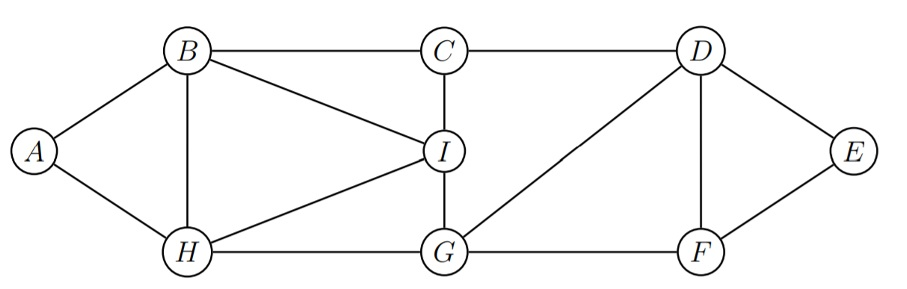
\includegraphics[scale=.74]{graph-image-v1.jpg}
\end{figure}


\begin{tabular}{|c|c|c|c|} \hline
  Vertex  & \hs\ \ha\  Color \hs\ \ha\ & \hs\  Distance \hs\ & \ha\ Predecessor \ha\  \\
  $v$ & $v.color$ & $v.d$ & $v.\pi$ \\ \hline
  A & & & \\ \hline
  B & & & \\ \hline
  C & & & \\ \hline
  D & & & \\ \hline
  E & & & \\ \hline
  F & & & \\ \hline
  G & & & \\ \hline
  H & & & \\ \hline
  I & & & \\ \hline
\end{tabular}
\vs\
\ls\
\end{document}
